\chapter{OPAMP Design and Verification}

\section{Architecture and schematic}

The core is a two-stage Miller-compensated OPAMP. M1/M2 form the NMOS differential pair, M3/M4 the PMOS current-mirror load, and M5 the tail-current source. The second stage uses PMOS M6 as a common-source device and NMOS M7 as its current-source load. M8 and the series bias resistors $R_0$/$R_2$ generate the bias voltage for M5 and M7. A series $R_Z$--$C_C$ branch from the first-stage node to the output provides frequency compensation.

\begin{figure}[htbp]
\centering
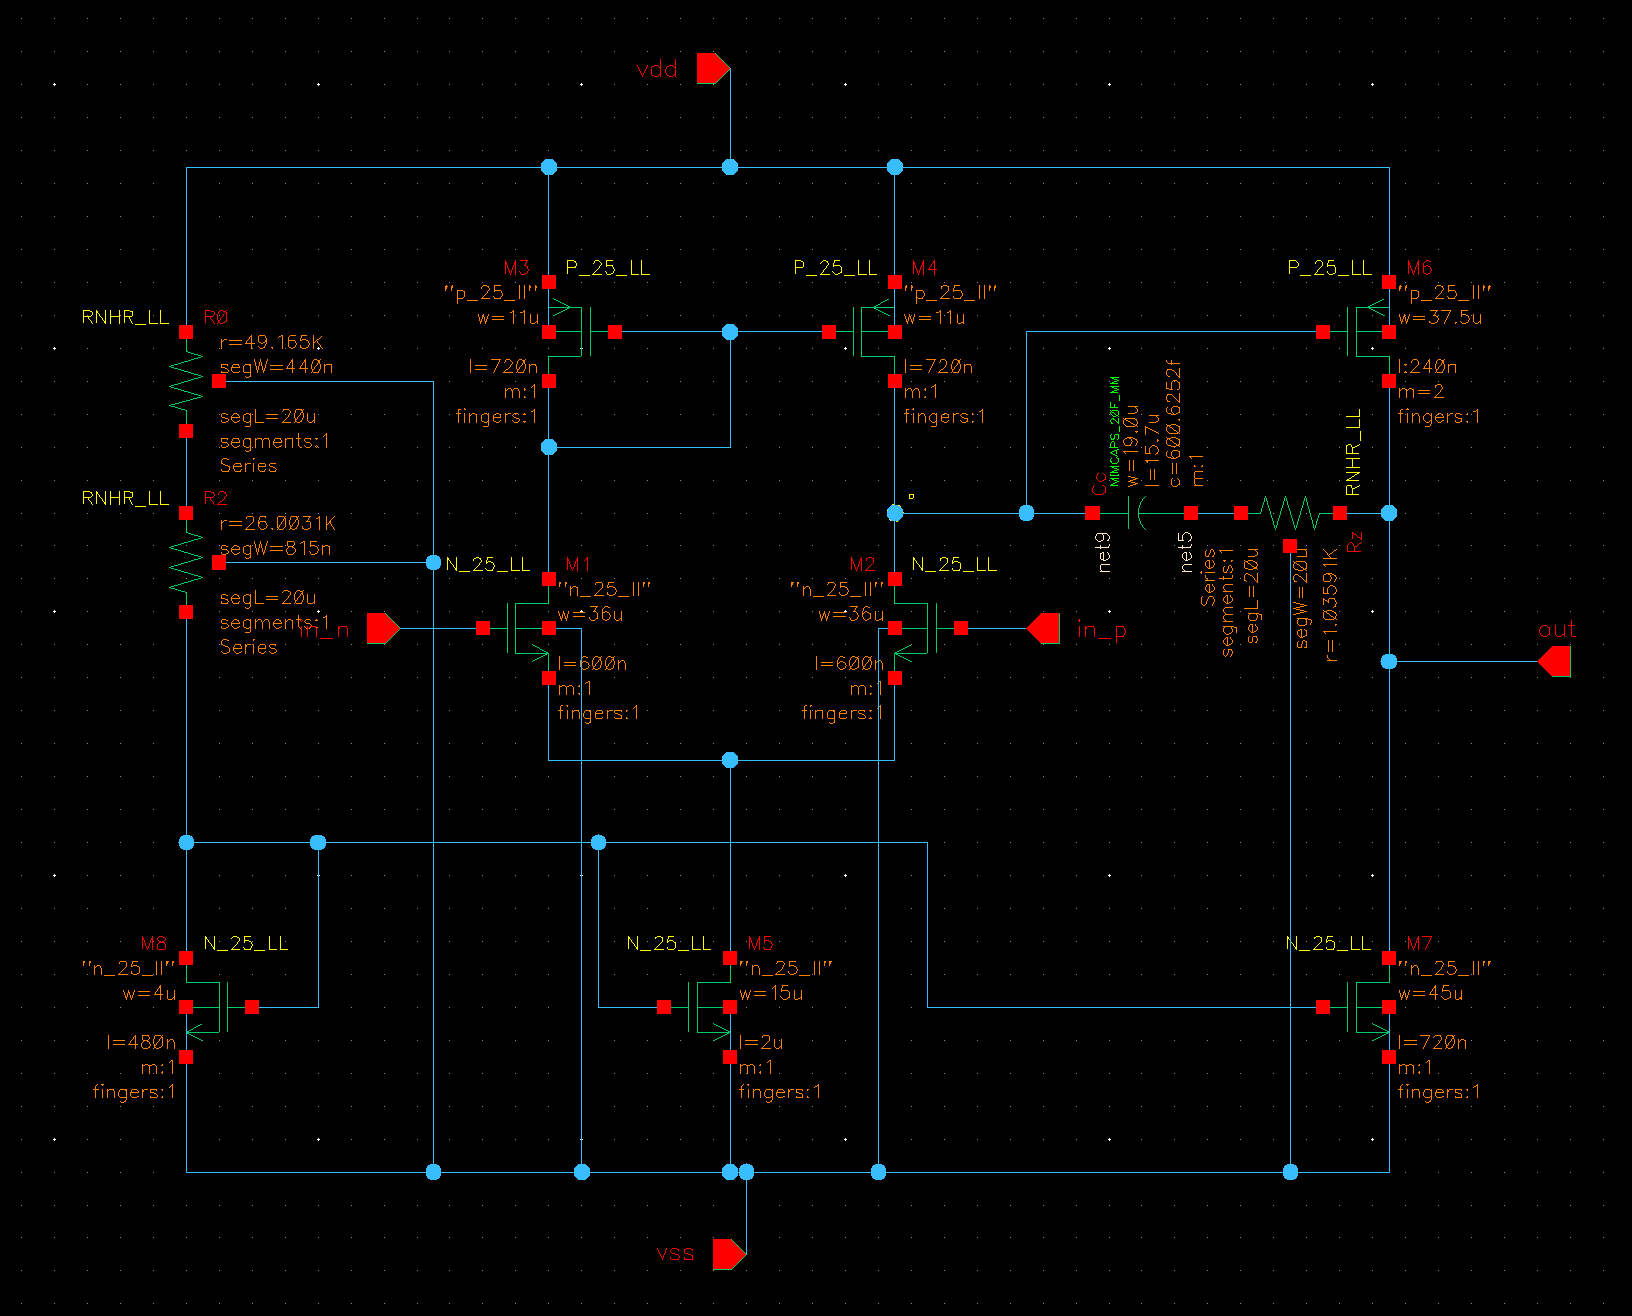
\includegraphics[width=\textwidth]{figures/opamp/schematic_final.png}
\caption{OPAMP schematic corresponding to the archived simulation baseline.}
\label{fig:final-schematic}
\end{figure}

The schematic interface is \texttt{in\_n}, \texttt{in\_p}, \texttt{out}, \texttt{vdd}, and \texttt{vss}. Figure~\ref{fig:final-schematic} shows the simulated schematic baseline. The verified results in this chapter use the same topology and interface together with the frozen schematic baseline values stated below, a \SI{1.8}{V} supply, a \SI{0.9}{V} input common-mode voltage, and a \SI{2}{pF} load.

\section{Hand calculation, sizing, and operating point}
\label{sec:final-design}

For the initial sizing, we fixed the channel length $L$, selected the target $g_m/I_D$, read the corresponding current density $I_D/W$, and calculated $W=I_D/(I_D/W)$. The hand calculation covers M1--M7; the M8 entry remains incomplete. Table~\ref{tab:sizing} compares these width targets with the first implementation and the final dimensions.

\begin{table}[htbp]
\centering
\caption{OPAMP sizing progression for the simulated schematic baseline (course Table~1). Dimensions are in \si{\micro m}; $L_{\min}=\SI{0.24}{\micro m}$.}
\label{tab:sizing}
\small
\resizebox{\textwidth}{!}{%
\begin{tabular}{@{}lrrrllr@{}}
\toprule
Device & Hand $g_m/I_D$ (V$^{-1}$) & Hand $I_D/W$ (\si{\micro A/\micro m}) & Hand $W$ target & First $W/L$ & Final effective $W/L$ & $L/L_{\min}$ \\
\midrule
M1/M2 & 17.049 & 1.555 & 5.145 & 24/0.48 & 36/0.60 & 2.50 \\
M3/M4 & 12.000 & 1.06130 & 7.538 & 7.34/0.48 & 11/0.72 & 3.00 \\
M5 & 13.010 & 1.5555 & 10.286 & 12.5/0.72 & 15/2.00 & 8.33 \\
M6 & 13.015 & 0.405 & 111.0 & 50/0.24 & 75/0.24 & 1.00 \\
M7 & 13.003 & 1.56775 & 29.98 & 45/0.72 & 45/0.72 & 3.00 \\
M8 & not completed & not completed & not completed & 4/0.48 & 4/0.48 & 2.00 \\
\bottomrule
\end{tabular}}

\vspace{0.6em}
\begin{tabularx}{\textwidth}{@{}l C C Y@{}}
\toprule
Parameter & Initial note/check & Final schematic & Interpretation \\
\midrule
$V_b$ & \SI{0.601}{V} & \SI{0.7354}{V} & diode-connected M8 gate/drain voltage \\
$C_C$ & \SI{1.464}{pF} first schematic & \SI{0.600625}{pF} & reduced during slew/stability tuning \\
$I_8$ & \SI{6.60}{\micro A} & \SI{14.18}{\micro A} & bias-reference branch \\
$I_5$ & \SI{7.11}{\micro A} & \SI{21.15}{\micro A} & input-pair tail current \\
$I_7$ & \SI{42.49}{\micro A} & \SI{137.6}{\micro A} & second-stage current \\
\bottomrule
\end{tabularx}
\end{table}

The bias resistance started as a single \SI{75}{k\ohm} element. The verified schematic baseline used $R_0\approx\SI{49.165}{k\ohm}$ and $R_2\approx\SI{26.003}{k\ohm}$. The compensation network uses approximately $R_Z=\SI{1.0359}{k\ohm}$ and $C_C=\SI{600.625}{fF}$. The numerical results remain tied to this schematic baseline.

Table~\ref{tab:op-point} summarizes selected values from the archived operating-point analysis. The full device-parameter export is omitted from this portfolio. All devices have positive $\lvert V_{DS}\rvert-\lvert V_{\mathrm{DSAT}}\rvert$. M5 has the smallest saturation margin, about \SI{65}{mV}, and is therefore the first device we would recheck after extraction.

\begin{table}[htbp]
\centering
\caption{Final nominal DC operating point from testbench instance \texttt{I38}. Currents are shown as absolute values.}
\label{tab:op-point}
\small
\begin{tabular}{@{}lrrrr@{}}
\toprule
Device & $\lvert I_D\rvert$ (\si{\micro A}) & $g_m/I_D$ (V$^{-1}$) & $r_o$ & Saturation margin (mV) \\
\midrule
M1/M2 & 10.60 / 10.54 & 21.87 / 21.88 & 2.004 / 2.097 M$\Omega$ & 809 / 904 \\
M3/M4 & 10.60 / 10.54 & 10.73 / 10.73 & 1.773 / 1.482 M$\Omega$ & 549 / 454 \\
M5 & 21.15 & 8.775 & 51.23 k$\Omega$ & 65 \\
M6 & 137.6 & 13.14 & 30.75 k$\Omega$ & 795 \\
M7 & 137.6 & 11.11 & 258.3 k$\Omega$ & 755 \\
M8 & 14.18 & 12.54 & 1.318 M$\Omega$ & 608 \\
\bottomrule
\end{tabular}
\end{table}

The nominal output is approximately \SI{0.9005}{V}. The total supply current is approximately \SI{172.9}{\micro A}, consistent with \SI{0.3113}{mW} at \SI{1.8}{V}.

\section{Design evolution and engineering decisions}

We increased the bias current to improve GBW and positive slew rate, but this raised power and reduced phase-margin and CMRR headroom. We therefore retained a bias resistance near \SI{75}{k\ohm} and tuned the device dimensions and compensation around these limits.

An effective M6 width of \SI{75}{\micro m} improved the phase margin. For M3/M4, $11/0.72$ gave better gain, CMRR, and noise. We rejected $22/1.44$ because its minimum CMRR was \SI{57.19}{dB} and its phase margin fell to \SI{51.84}{\degree}; a wider M7 was also rejected because it increased power and reduced negative slew rate.

For M5, $12/2.0$ improved small-signal behavior but reduced the slew rates. SR+ fell to approximately \SI{14.5}{V/\micro s} and SR$-$ to \SI{8.79}{V/\micro s}, so we retained $15/2.0$. Reducing $C_C$ improved negative slew rate but reduced stability; the series $R_Z$ recovered phase margin. We finally set $C_C\approx\SI{0.60}{pF}$ and $R_Z\approx\SI{1}{k\ohm}$ as a balance among bandwidth, stability, slew rate, noise, and power.

\section{Testbench and measurements}

Separate testbench instances cover offset, open-loop gain/CMRR, ICMR, output swing, power, slew/settling, input-referred noise, and stability, as shown in Figure~\ref{fig:testbench}. This keeps the stimuli independent and the output expressions easy to check.

% TODO(figure readability): Replace this full-window screenshot with two larger crops if a higher-resolution Cadence export becomes available. The present image documents the testbench topology, but small component annotations are not legible at print scale.
\begin{figure}[htbp]
\centering
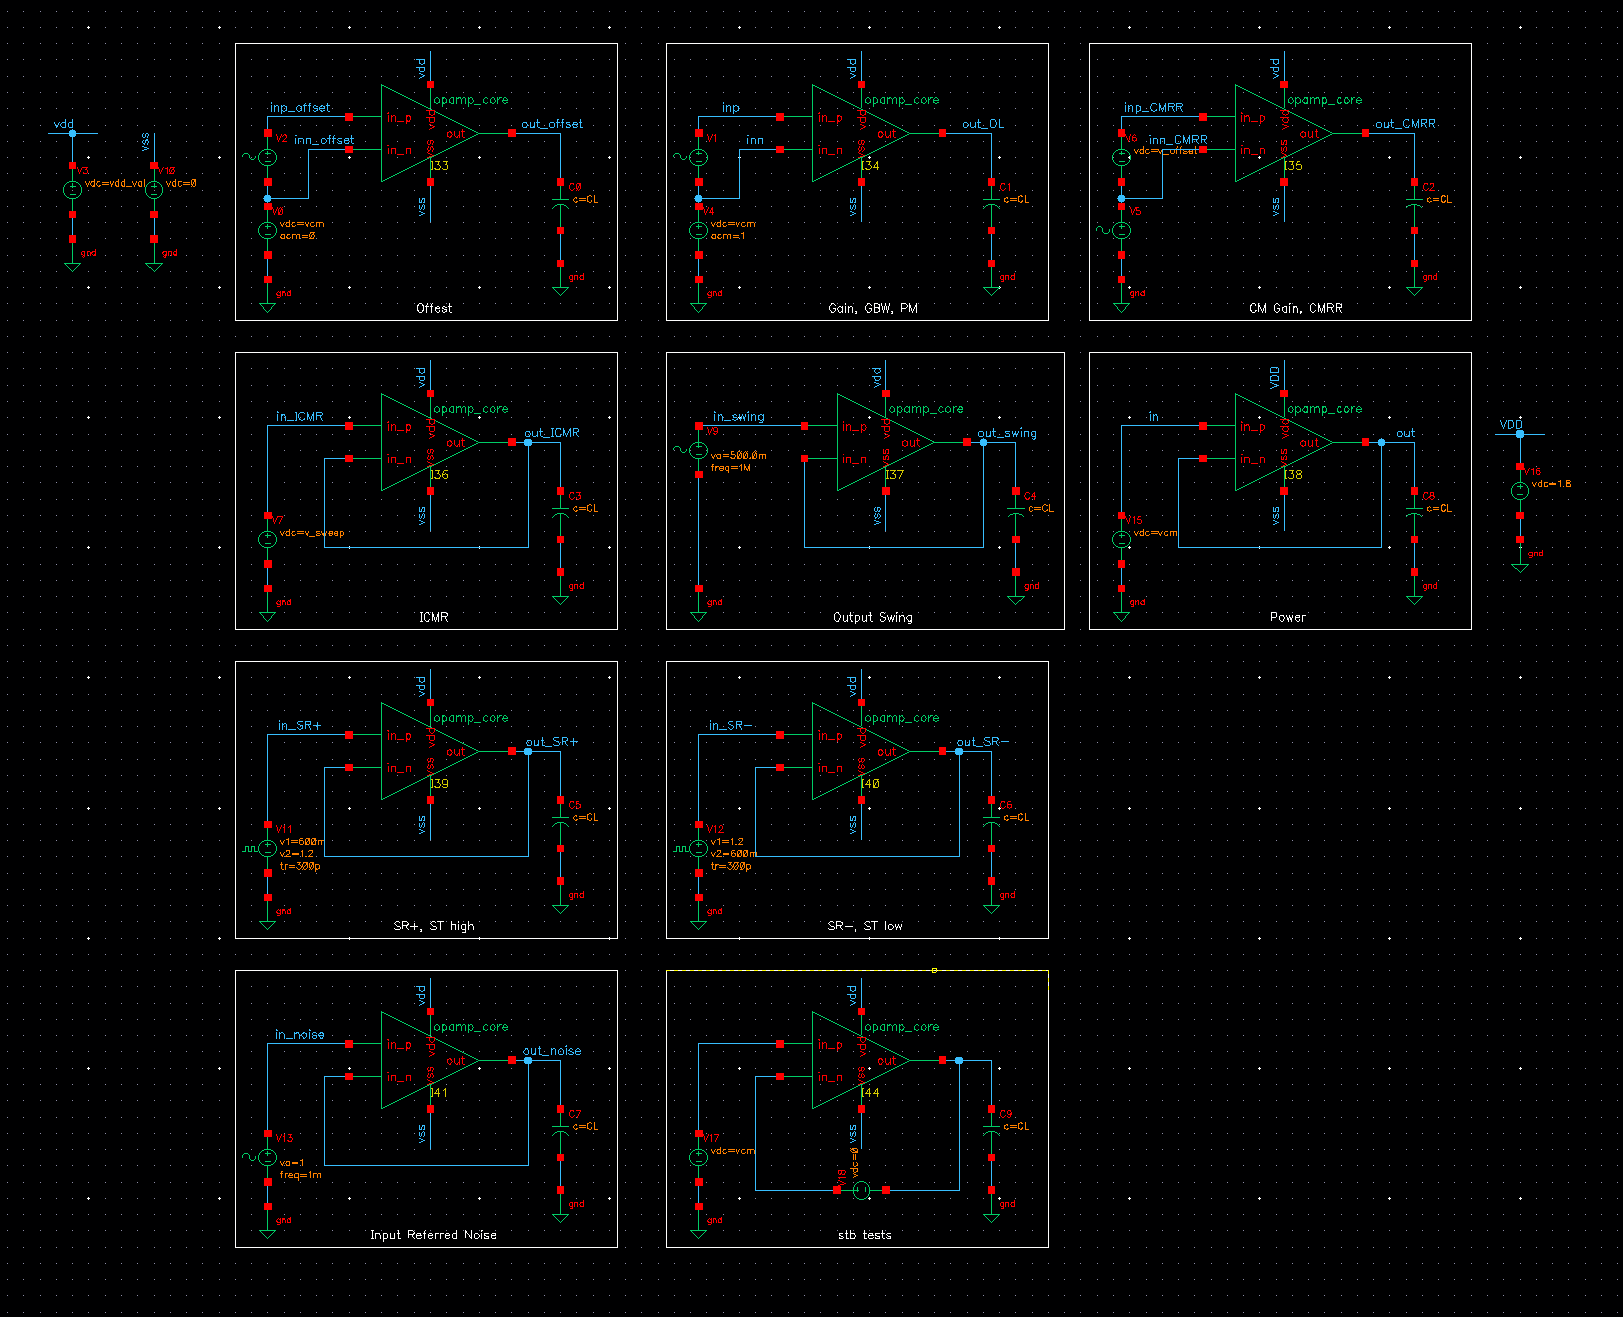
\includegraphics[width=\textwidth]{figures/opamp/testbench_final.png}
\caption{Schematic-level OPAMP testbenches for offset, AC/stability, CMRR, ICMR, output swing, power, slew/settling, and input noise. Each simulated output uses a \SI{2}{pF} load.}
\label{fig:testbench}
\end{figure}

The AC sweep covers \SI{1}{Hz}--\SI{1}{GHz} with 80 points per decade, while the noise sweep covers \SI{1}{Hz}--\SI{100}{MHz}; transient simulations run for \SI{1}{\micro s}. Slew and settling use \SI{0.6}{V}/\SI{1.2}{V} pulses with \SI{300}{ps} edges. The output-swing test uses a unity follower driven by \SI{0.9}{V} $\pm$ \SI{0.5}{V} at \SI{1}{MHz}.

\section{Nominal results}

Nominal simulations use TT/typical models at \SI{27}{\degreeCelsius}, \(\VDD=\SI{1.8}{V}\), \(\VCM=\SI{0.9}{V}\), and a \SI{2}{pF} load. The reported temperature is the exported simulation value.

% LAYOUT HANDOFF: Fill the Post-layout column from the extracted-view run and
% add a separate PEX pass/fail entry if the final table format is adjusted.
% Keep every schematic value unchanged. See ../../docs/verification.md.

\begin{table}[H]
\centering
\caption{Nominal OPAMP results with a \SI{2}{pF} load (course Table~2). Post-layout entries remain unavailable because no extracted-view simulation output was supplied.}
\label{tab:nominal-spec}
\small
\resizebox{\textwidth}{!}{%
\begin{tabular}{@{}llllll@{}}
\toprule
Metric & Requirement & Schematic nominal & Status & Post-layout & Simulation output \\
\midrule
DC gain & $>50$ dB & 79.93 dB & Pass & -- & ADE scalar \\
GBW & $\geq20$ MHz & 51.31 MHz & Pass & -- & ADE scalar \\
Phase margin & $\geq55^\circ$ & $61.97^\circ$ & Pass & -- & ADE scalar \\
CMRR & $>60$ dB & 68.53 dB & Pass & -- & ADE scalar \\
SR+ / SR$-$ & $\geq15/15$ V/\si{\micro s} & 35.17 / 27.43 V/\si{\micro s} & Pass & -- & transient scalars \\
Settling high / low (5\%) & $\leq500/500$ ns & 16.39 / 23.17 ns & Pass & -- & transient scalars \\
ICMR & 0.5--1.3 V & 0.8503 mV max. error & Pass & -- & clipped follower sweep \\
Output swing & 0.3--1.5 V & 0.4302--1.4006 V & Does not meet & -- & follower transient \\
Input offset & $\leq5$ mV abs. & $-0.4516$ mV & Pass & -- & ADE scalar \\
Noise at 20 kHz & $\leq55$ nV/$\sqrt{\mathrm{Hz}}$ & 32.78 nV/$\sqrt{\mathrm{Hz}}$ & Pass & -- & scalar and marker \\
Power & $\leq0.6$ mW & 0.3113 mW & Pass & -- & ADE scalar \\
Area & report value & n/a & n/a & -- & no scaled layout export \\
\bottomrule
\end{tabular}}
\end{table}

For the ICMR check, we configured the OPAMP as a unity-gain follower and swept the non-inverting input from \SI{0}{V} to \SI{1.8}{V}. The ADE expression clips the waveform to the required \SIrange{0.5}{1.3}{V} interval before taking the maximum error:
\begin{equation}
\varepsilon_{\mathrm{ICMR,max}}
=\max_{0.5\,\mathrm{V}\leq V_{\mathrm{in}}\leq1.3\,\mathrm{V}}
\left|V_{\mathrm{out}}(V_{\mathrm{in}})-V_{\mathrm{in}}\right|
=\SI{850.3}{\micro V}.
\end{equation}
The resulting \SI{0.8503}{mV} maximum error is well below the \SI{50}{mV} limit. This verifies the specified ICMR interval with the stated follower-error criterion; the wider \SIrange{0}{1.8}{V} sweep is only the test range and is not reported as the ICMR.

The simulated output swing is approximately \SIrange{0.430}{1.401}{V}, with raw limits of \SI{0.430203}{V} and \SI{1.40056}{V}. This does not cover the full specified \SIrange{0.3}{1.5}{V} range. We retained the circuit because earlier changes reduced the available margins in stability, slew rate, CMRR, noise, or power. The limitation caused no failure in the available PGA corner or Monte Carlo runs under their applied stimuli, although those runs do not turn the swing result into a specification pass.

The input-noise scalar is \SI{32.7766}{nV}/$\sqrt{\mathrm{Hz}}$. At \SI{20}{kHz}, the waveform marker reads \SI{32.8072}{nV}/$\sqrt{\mathrm{Hz}}$. The \SI{0.0306}{nV}/$\sqrt{\mathrm{Hz}}$ difference is consistent with display and sampling precision and supports the rounded \SI{32.78}{nV}/$\sqrt{\mathrm{Hz}}$ result in Tables~\ref{tab:nominal-spec} and \ref{tab:corners}.

% TODO(figure readability): Replace the nominal overview with larger individual crops if new exports are available. The present composite documents the waveform set, while exact values are taken from the tables and scalar outputs.
\begin{figure}[p]
\centering
\textbf{(a) Nominal overview}\par\smallskip
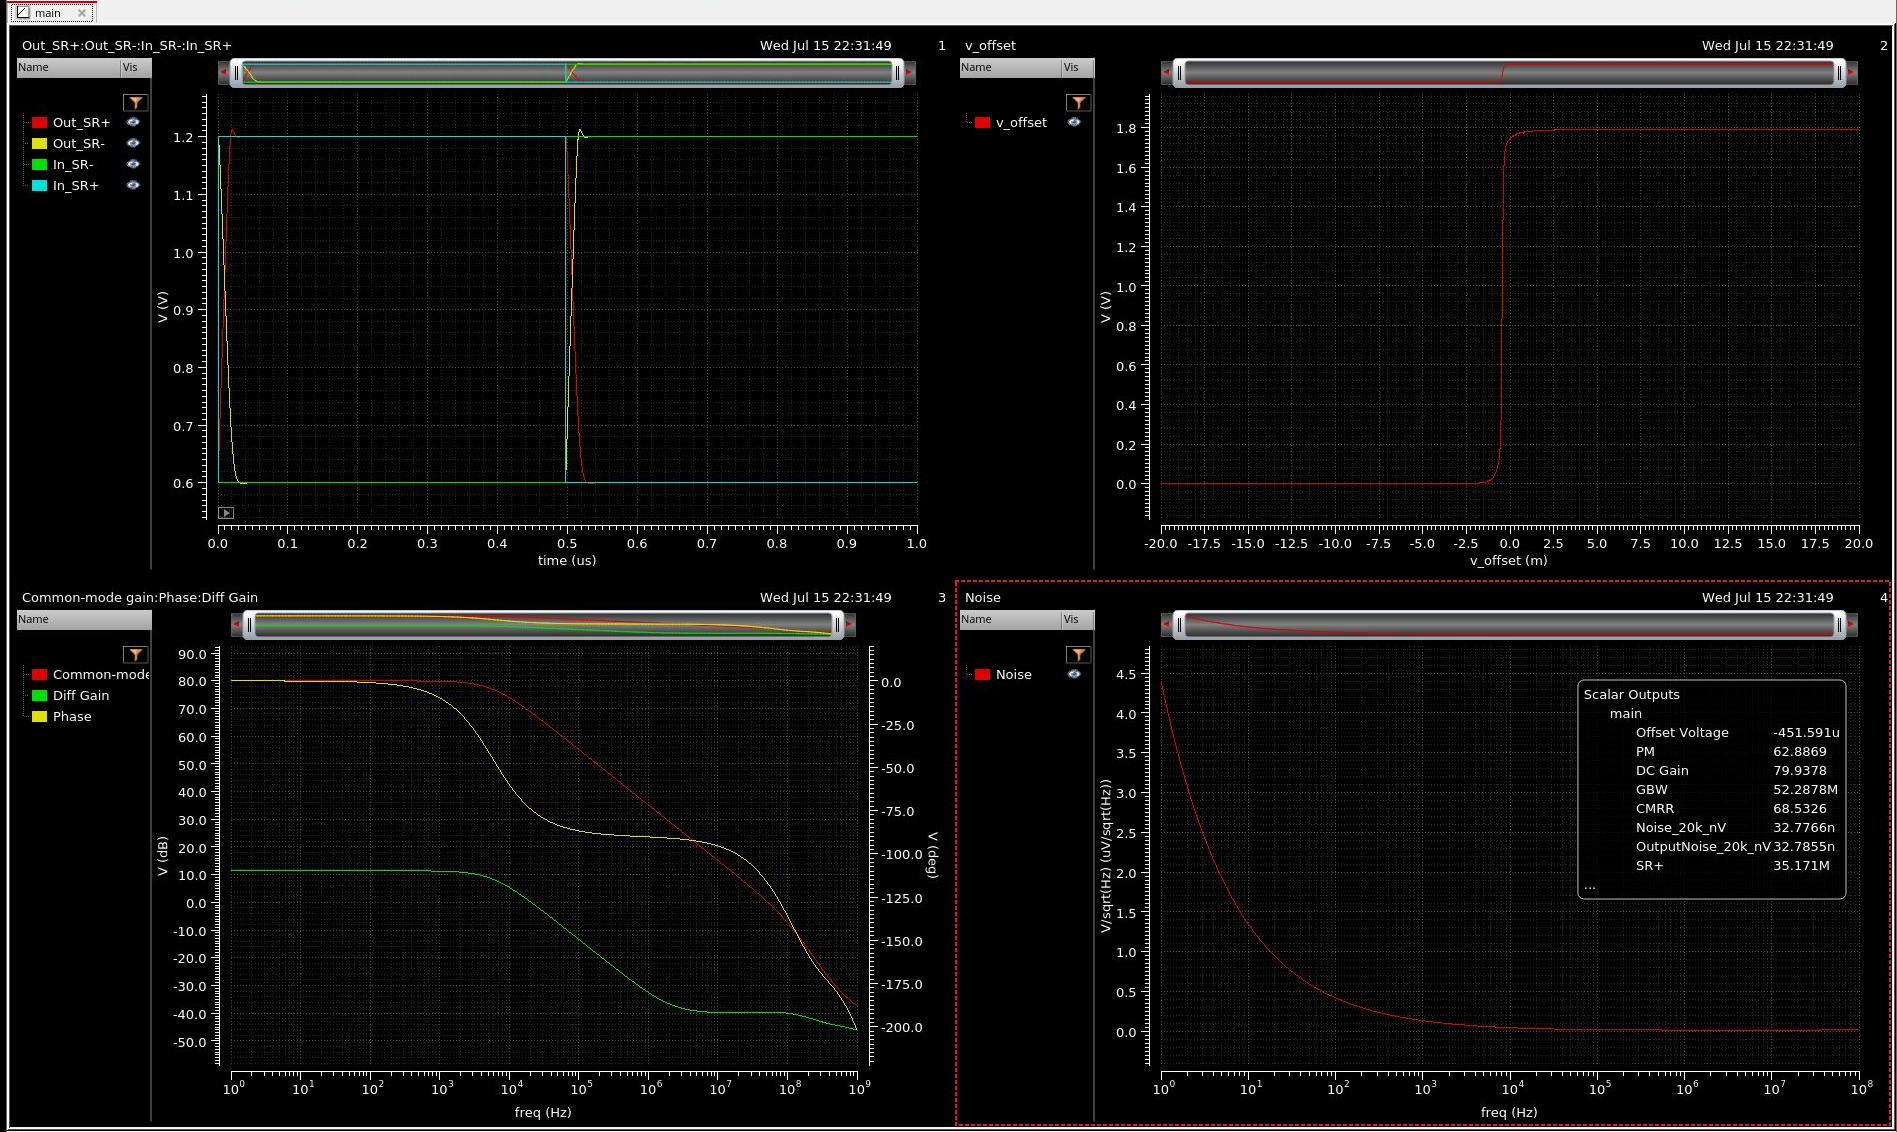
\includegraphics[width=0.66\textwidth]{figures/opamp/nominal_overview.png}

\smallskip
\textbf{(b) ICMR criterion and result}\par\smallskip
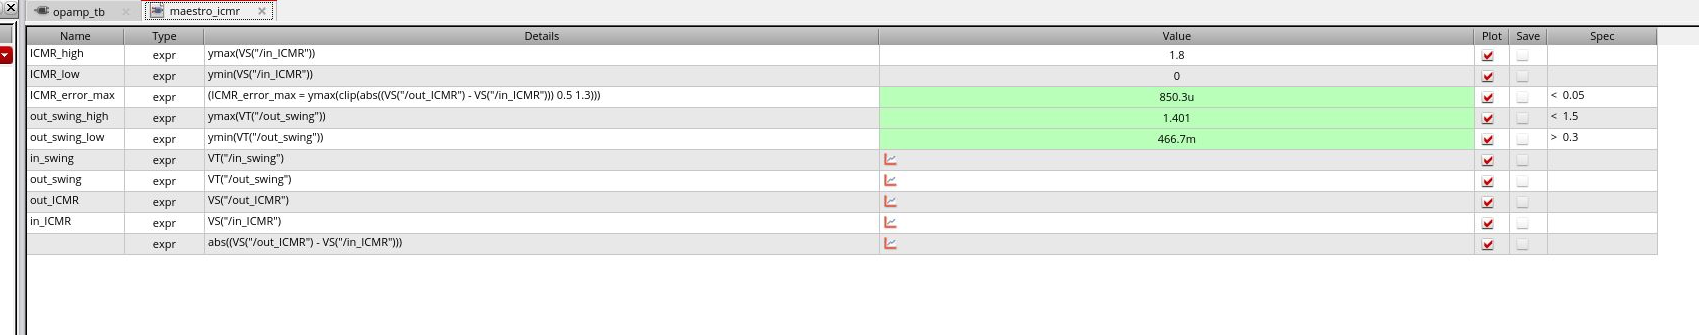
\includegraphics[width=0.96\textwidth,trim=0 225 470 0,clip]{figures/opamp/icmr_expression.png}

\smallskip
\begin{minipage}[t]{0.31\textwidth}
\centering
\textbf{(c) Output swing}\par\smallskip
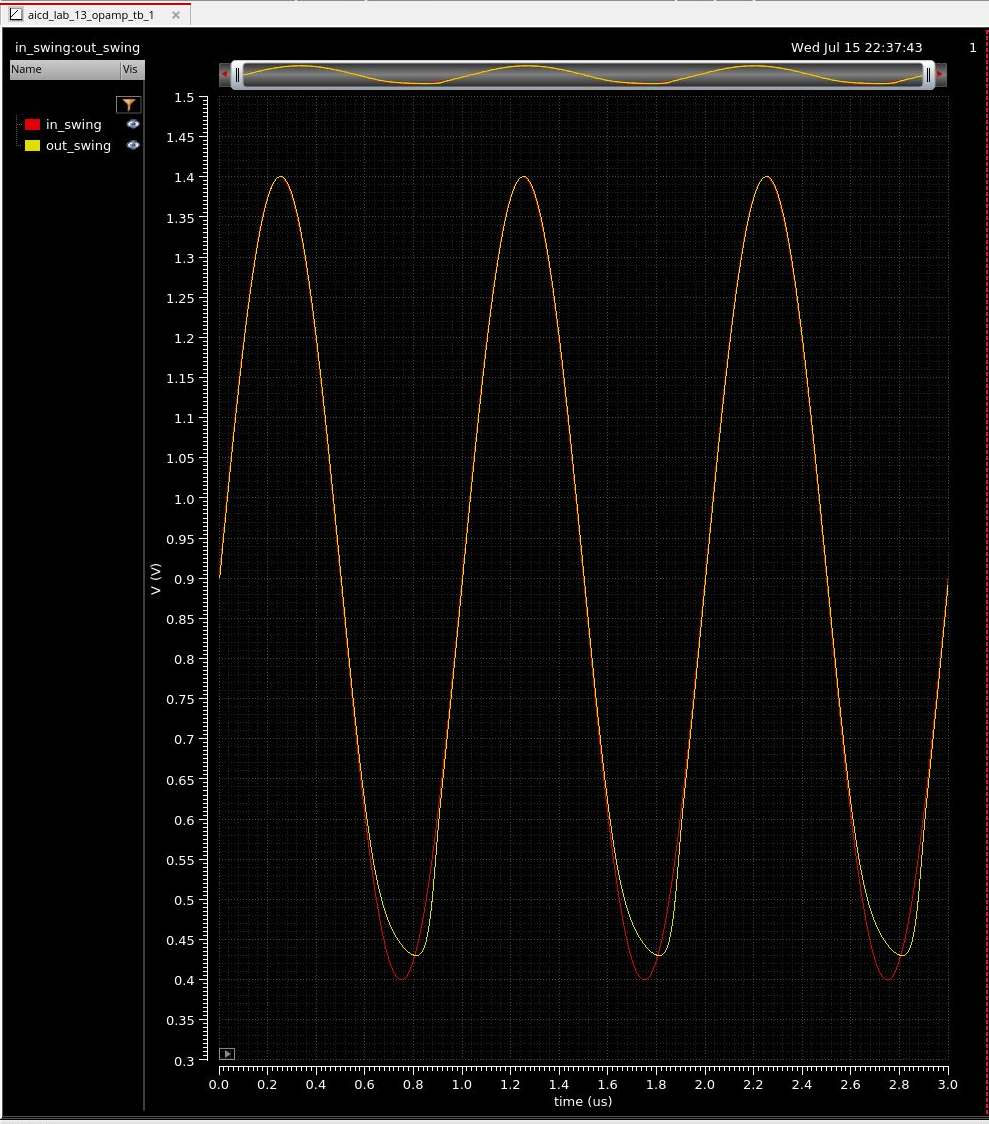
\includegraphics[width=\linewidth]{figures/opamp/output_swing.png}
\end{minipage}\hspace{0.035\textwidth}
\begin{minipage}[t]{0.41\textwidth}
\centering
\textbf{(d) Input noise at \SI{20}{kHz}}\par\smallskip
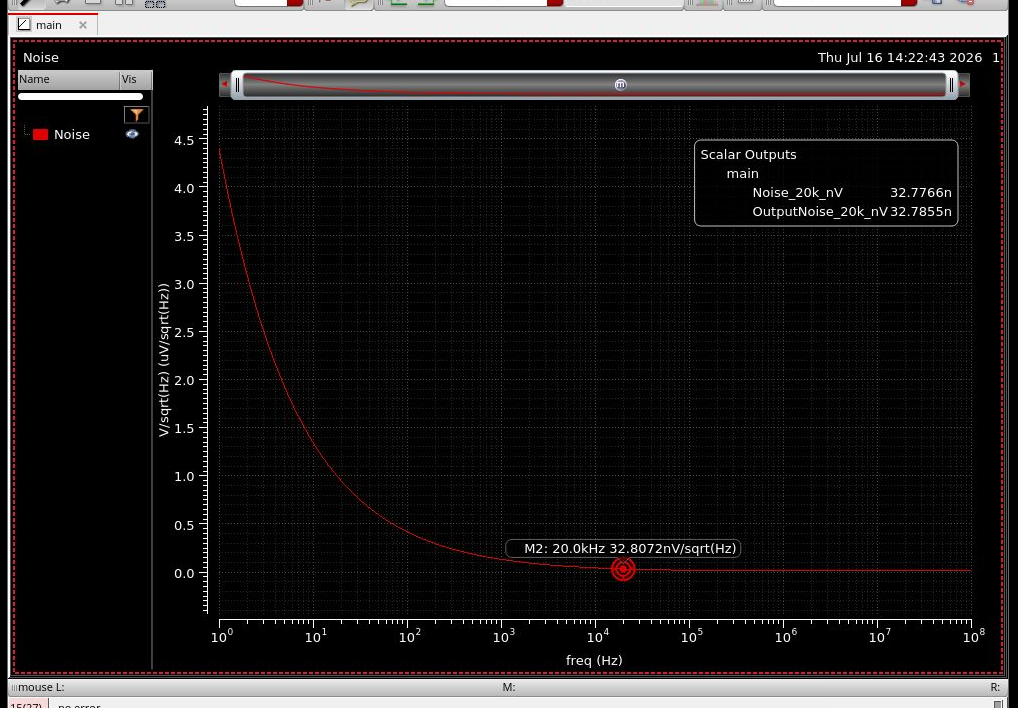
\includegraphics[width=\linewidth]{figures/opamp/noise_20k.png}
\end{minipage}
\caption{Nominal OPAMP simulations: (a) response overview, (b) clipped ICMR follower-error expression and scalar result, (c) output-swing transient, and (d) input-noise spectrum with a \SI{20}{kHz} marker. Exact values are reported in Table~\ref{tab:nominal-spec}.}
\label{fig:opamp-key-plots}
\end{figure}

\section{PVT-corner results}

The PVT sweep combines two MIM sections, two resistor sections, four device/process sections, two temperatures (\SI{-25}{\degreeCelsius}, \SI{85}{\degreeCelsius}), and two supplies (\SI{1.62}{V}, \SI{1.98}{V}):
\begin{equation}
N_{\mathrm{corner}}=2\times2\times4\times2\times2=64.
\end{equation}

Every one of the 12 output expressions included in the export is marked \texttt{pass}. Table~\ref{tab:corners} therefore reports 64/64 directly from the raw CSV. ICMR and output swing are not part of this corner export; the all-pass statement does not cover them.

% LAYOUT HANDOFF: For the final report, write each PEX value first and the
% schematic value in parentheses. Report the PEX and schematic pass counts
% separately, e.g. 64 (64)/64. Do not extend the claim to ICMR or swing unless
% those expressions are explicitly added to the extracted-view sweep.

\begin{table}[H]
\centering
\caption{PVT-corner summary with a \SI{2}{pF} load (course Table~3).}
\label{tab:corners}
\small
\resizebox{\textwidth}{!}{%
\begin{tabular}{@{}lrrrrrl@{}}
\toprule
Metric & Requirement & Nominal & Minimum & Maximum & Passed/total & Limiting corner \\
\midrule
DC gain (dB) & $>50$ & 79.93 & 76.32 & 82.76 & 64/64 & C9, minimum \\
GBW (MHz) & $\geq20$ & 51.31 & 32.28 & 72.94 & 64/64 & C57, minimum \\
Phase margin ($^\circ$) & $\geq55$ & 61.97 & 59.57 & 68.81 & 64/64 & C4, minimum \\
CMRR (dB) & $>60$ & 68.53 & 61.54 & 74.50 & 64/64 & C26, minimum \\
SR+ (V/\si{\micro s}) & $\geq15$ & 35.17 & 22.34 & 49.14 & 64/64 & C41, minimum \\
SR$-$ (V/\si{\micro s}) & $\geq15$ & 27.43 & 16.04 & 34.90 & 64/64 & C56, minimum \\
Settling high (ns) & $\leq500$ & 16.39 & 11.77 & 26.36 & 64/64 & C41, maximum \\
Settling low (ns) & $\leq500$ & 23.17 & 18.11 & 41.74 & 64/64 & C56, maximum \\
Offset (mV) & $\lvert\cdot\rvert\leq5$ & $-0.4516$ & $-0.7204$ & $-0.2660$ & 64/64 & C41, max. absolute \\
Noise (nV/$\sqrt{\mathrm{Hz}}$) & $\leq55$ & 32.78 & 29.17 & 45.73 & 64/64 & C49, maximum \\
Power (\si{\micro W}) & $\leq600$ & 311.3 & 266.3 & 367.8 & 64/64 & C9, maximum \\
\bottomrule
\end{tabular}}
\end{table}

The closest numeric limits are SR$-$ with \SI{1.04}{V/\micro s} headroom, CMRR with \SI{1.54}{dB}, and phase margin with \SI{4.57}{\degree}. The worst noise value still has \SI{9.27}{nV}/$\sqrt{\mathrm{Hz}}$ of headroom. The raw export identifies C56 as the slow-resistor/slow-process, \SI{-25}{\degreeCelsius}, \SI{1.62}{V} point; C26 limits CMRR, and C4 limits phase margin.

\section{Schematic Monte Carlo analysis}

The Monte Carlo analysis uses variation \texttt{All}, 1000 points, standard random sampling, seed 12345, and first point 1. Separate transient, offset, and stability tests provide 1000 samples for each reported metric.

% LAYOUT HANDOFF: Add the 1000-point extracted-view statistics in the form
% PEX (schematic), including yield. Do not replace the 972/1000 schematic
% offset yield. See ../../docs/verification.md.

\begin{table}[H]
\centering
\caption{OPAMP Monte Carlo summary, 1000 samples per test (course Table~4).}
\label{tab:mc}
\small
\resizebox{\textwidth}{!}{%
\begin{tabular}{@{}lrrrrrrl@{}}
\toprule
Metric & Minimum & Maximum & Mean & $\sigma$ & Yield & Errors & Status \\
\midrule
DC gain (dB) & 79.09 & 80.75 & 79.93 & 0.2452 & 1000/1000 & 0 & Pass \\
GBW (MHz) & 42.09 & 63.05 & 51.42 & 3.250 & 1000/1000 & 0 & Pass \\
Phase margin ($^\circ$) & 56.28 & 66.40 & 61.93 & 1.479 & 1000/1000 & 0 & Pass \\
SR+ (V/\si{\micro s}) & 27.06 & 44.66 & 35.16 & 2.742 & 1000/1000 & 0 & Pass \\
SR$-$ (V/\si{\micro s}) & 21.82 & 35.37 & 27.43 & 2.072 & 1000/1000 & 0 & Pass \\
Settling high (ns) & 12.94 & 21.31 & 16.48 & 1.282 & 1000/1000 & 0 & Pass \\
Settling low (ns) & 17.94 & 29.65 & 23.31 & 1.786 & 1000/1000 & 0 & Pass \\
Offset (mV) & $-7.447$ & 5.518 & $-0.4735$ & 2.212 & 972/1000 & 0 & 97.2\% \\
\bottomrule
\end{tabular}}
\end{table}

Offset is the only reported metric with less than 100\% yield. Its mean is \SI{-0.474}{mV}, and 28 of 1000 samples exceed the \SI{5}{mV} absolute limit, giving 972/1000.

\begin{figure}[htbp]
\centering
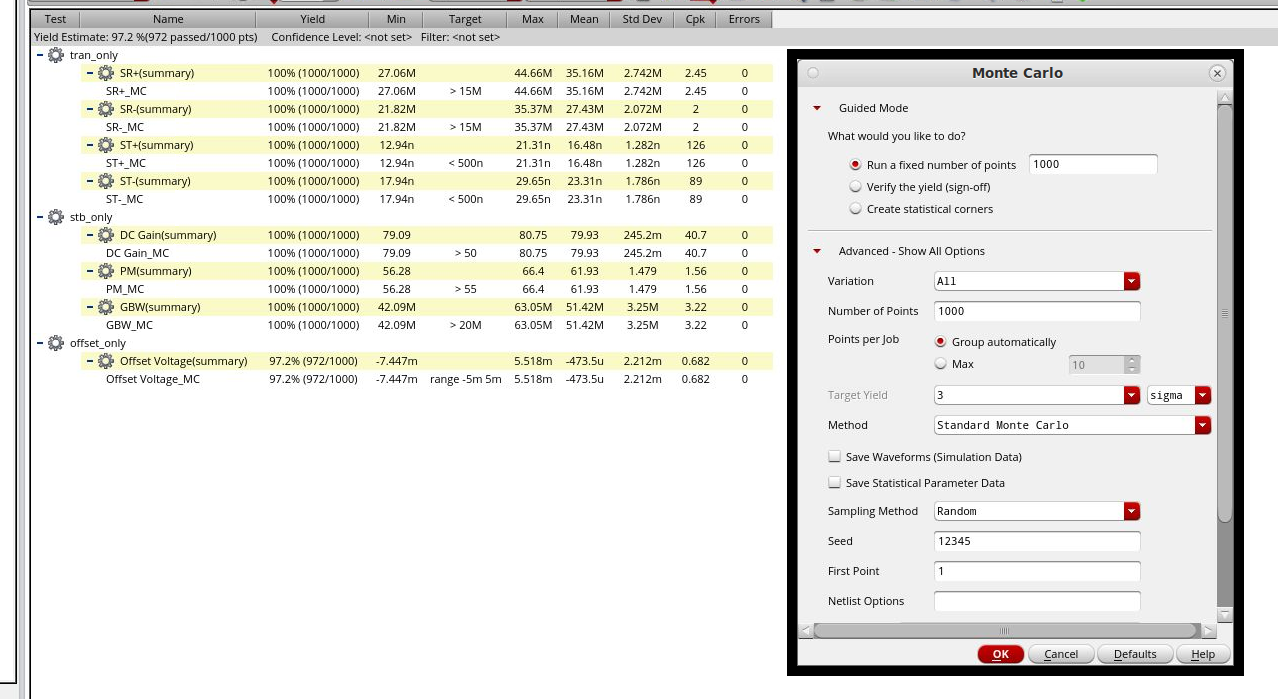
\includegraphics[width=\textwidth]{figures/opamp/mc_summary.png}
\caption{ADE Monte Carlo summary and sampling setup for variation \texttt{All}, 1000 samples per test, random sampling, and seed 12345.}
\label{fig:mc-summary}
\end{figure}
